%  !TeX  root  =  user_guide.tex 

\section{Plugin Georeferenziatore}\label{sec:georef}

% when the revision of a section has been finalized, 
% comment out the following line:
% \updatedisclaimer

Il Plugin Georeferenziatore è uno strumento per generare file di georeferenziazione (world file) per i raster. 
Permette di georeferenziare raster in sistemi di coordinate geografiche e proiettate, creando un GeoTiff oppure 
associandogli un world file. L'approccio di base del plugin è quello di individuare punti del raster per i 
quali sia possibile determinare accuratamente le coordinate.

\minisec{Features}

\begin{table}[h]\index{Georeferenziatore!strumenti}
\begin{tabular}{|m{1cm}|m{6cm}|m{1cm}|m{6cm}|}
	\hline \textbf{Icona} & \textbf{Azione} & \textbf{Icona} &
 \textbf{Azione} \\
 \hline 
\includegraphics[width=0.7cm]{mActionAddRasterLayer} & Carica un raster &
 
\includegraphics[width=0.7cm]{mActionStartGeoref} & Avvia la georeferenziazione \\
 \hline 
\includegraphics[width=0.7cm]{mActionGDALScript} & Genera uno script GDAL &
 
\includegraphics[width=0.7cm]{mActionFileOpen} & Carica punti CGP (Ground Control Point) \\
 \hline 
\includegraphics[width=0.7cm]{mActionFileSave} & Salva punti GCP come... &
 
\includegraphics[width=0.7cm]{mActionOptions} & Imposta la trasformazione \\
 \hline 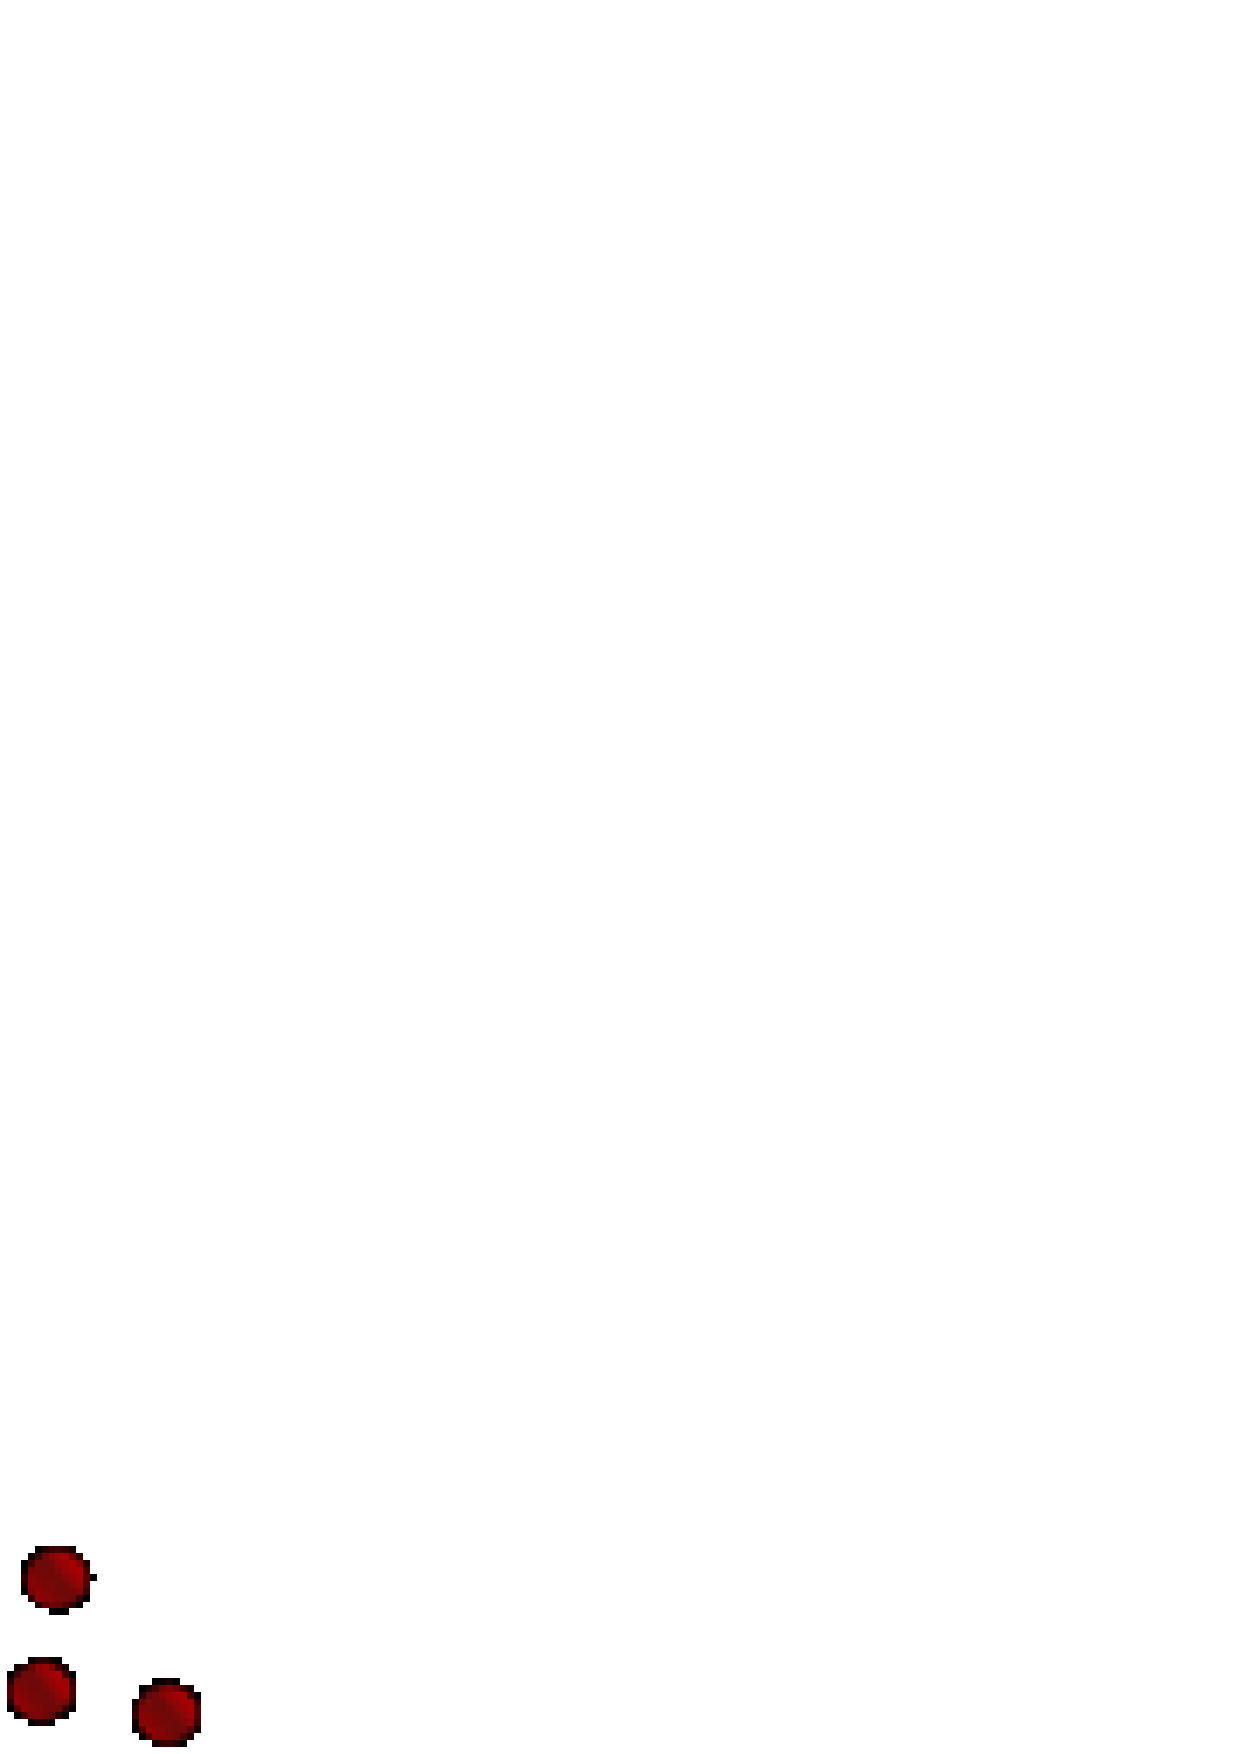
\includegraphics[width=0.7cm]{mActionCapturePoint} & Aggiunge un nuovo punto &
 
\includegraphics[width=0.7cm]{mActionDeleteSelected} & Elimina un punto \\
 \hline 
\includegraphics[width=0.7cm]{mActionMoveFeature} & Sposta un punto GCP &
 
\includegraphics[width=0.7cm]{mActionPan} & Sposta la vista \\
 \hline 
\includegraphics[width=0.7cm]{mActionZoomIn} & Ingrandisce al vista &
 
\includegraphics[width=0.7cm]{mActionZoomOut} & Rimpicciolisce la vista \\
 \hline 
\includegraphics[width=0.7cm]{mActionZoomToLayer} & Zoom sul layer &
 
\includegraphics[width=0.7cm]{mActionZoomLast} & Zoom precedente \\
 \hline 
\includegraphics[width=0.7cm]{mActionZoomNext} & Zoom successivo &
 
\includegraphics[width=0.7cm]{mActionLinkGeorefToQGis} & Collega il georeferenziatore a QGIS \\
 \hline 
\includegraphics[width=0.7cm]{mActionLinkQGisToGeoref} & Collega QGIS al georeferenziatore  &
 &  \\
\hline
\end{tabular}
\caption{Strumenti del georeferenziatore}\label{tab:georeferencer_tools}
\end{table}

\minisec{Utilizzo del plugin}

Per le coordinate dei punti selezionati sull'immagine possono essere usate due procedure alternative:

\begin{enumerate}
\item Inserire manualmente le coordinate: solitamente nei raster sono presenti 
punti con le coordinate scritte sull'immagine.
\item Usare un layer già georiferito (vettoriale o raster) contenente le stesse entità/oggetti 
del raster da georiferire. In questo caso le coordinate vengono inserire cliccando sul layer 
di riferimento nella vista mappa.
\end{enumerate}

Una procedura meno usuale consiste nel selezionare più punti del raster, specificarne le coordinate 
e scegliere un metodo di trasformazione. Sulla base dei parametri inseriti, il plugin 
calcola i parametri del world file. Più coordinate vengono fornite, migliore sarà il 
risultato.

Avviare QGIS, caricare il plugin (Sezione \ref{sec:load_core_plugin}) e cliccare 
sull'icona \toolbtntwo{georeferencer}{Georeferenziatore} nella barra dei plugin. 
Si aprirà la finestra di dialogo Georeferenziatore mostrata in Figura \ref{fig:georefplugin}.
  
Come esempio si può provare a georiferire carta topografica del South Dakota scaricabile da:
\url{http://grass.osgeo.org/sampledata/spearfish\_toposheet.tar.gz}

\begin{figure}[ht]
\centering
  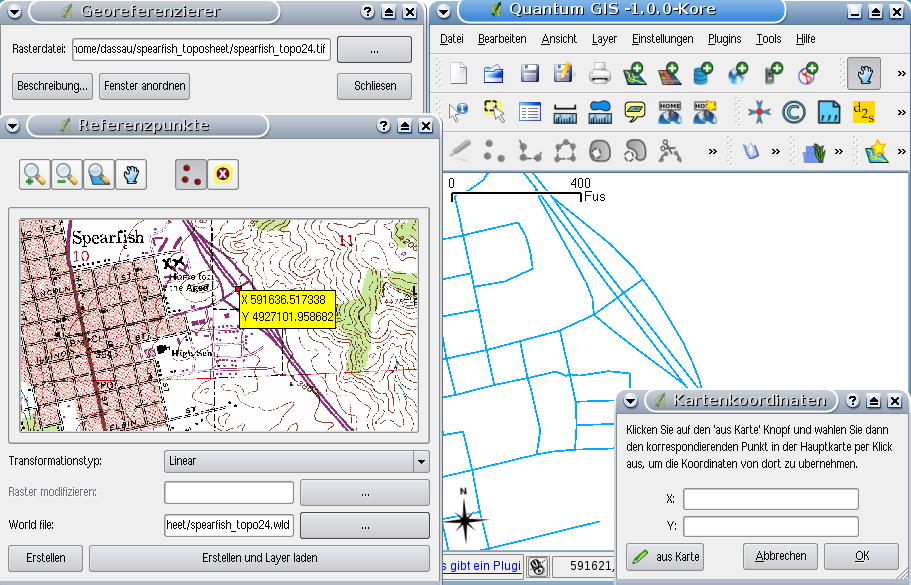
\includegraphics[clip=true, width=12cm]{georefplugin}
  \caption{Finestra di dialogo Georeferenziatore \nixcaption}\label{fig:georefplugin}
\end{figure}

\minisec{Aggiungere punti GCP}\label{georeferencer_entering}

\begin{enumerate}
\item Per iniziare a georiferire un raster, caricarlo cliccando sul pulsante

\includegraphics[width=0.7cm]{mActionAddRasterLayer}{Apri raster}: il raster 
sarà visualizzato  nel riquadro principale della finestra di dialogo.
Caricato il raster, è ora possibile iniziare ad inserire i punti di riferimento.
\item Usare il pulsante \toolbtntwo{mActionCapturePoint}{Aggiunti punto} per 
aggiungere punti sul raster ed inserirne le coordinare (Figura \ref{fig:choose_points}). 
Per inserire le coordinate si hanno due opzioni:

\begin{enumerate}
\item Cliccare su un punto del raster ed inserire le coordinate X/Y manualmente.
\item Cliccare su un punto del raster ed usare il pulsante \toolbtntwo{pencil}{Dalla mappa} 
per inserire le coordinate X/Y con l'aiuto di layer già georeferenziato caricato 
nella vista mappa di QGIS.
\item Se necessario usare il pulsante 
\includegraphics[width=0.7cm]{mActionMoveFeature}{Muovi punto GCP}
per spostare i punti in entrambe le finestre.
\end{enumerate}
\item Bisogna inserire almeno 4 GCP: più punti vengono inseriti, migliore sarà il risultato. 
Aiutarsi con gli altri strumenti del plugin per spostarsi nell'area di lavoro.
\end{enumerate}

\begin{figure}[ht]
\centering
  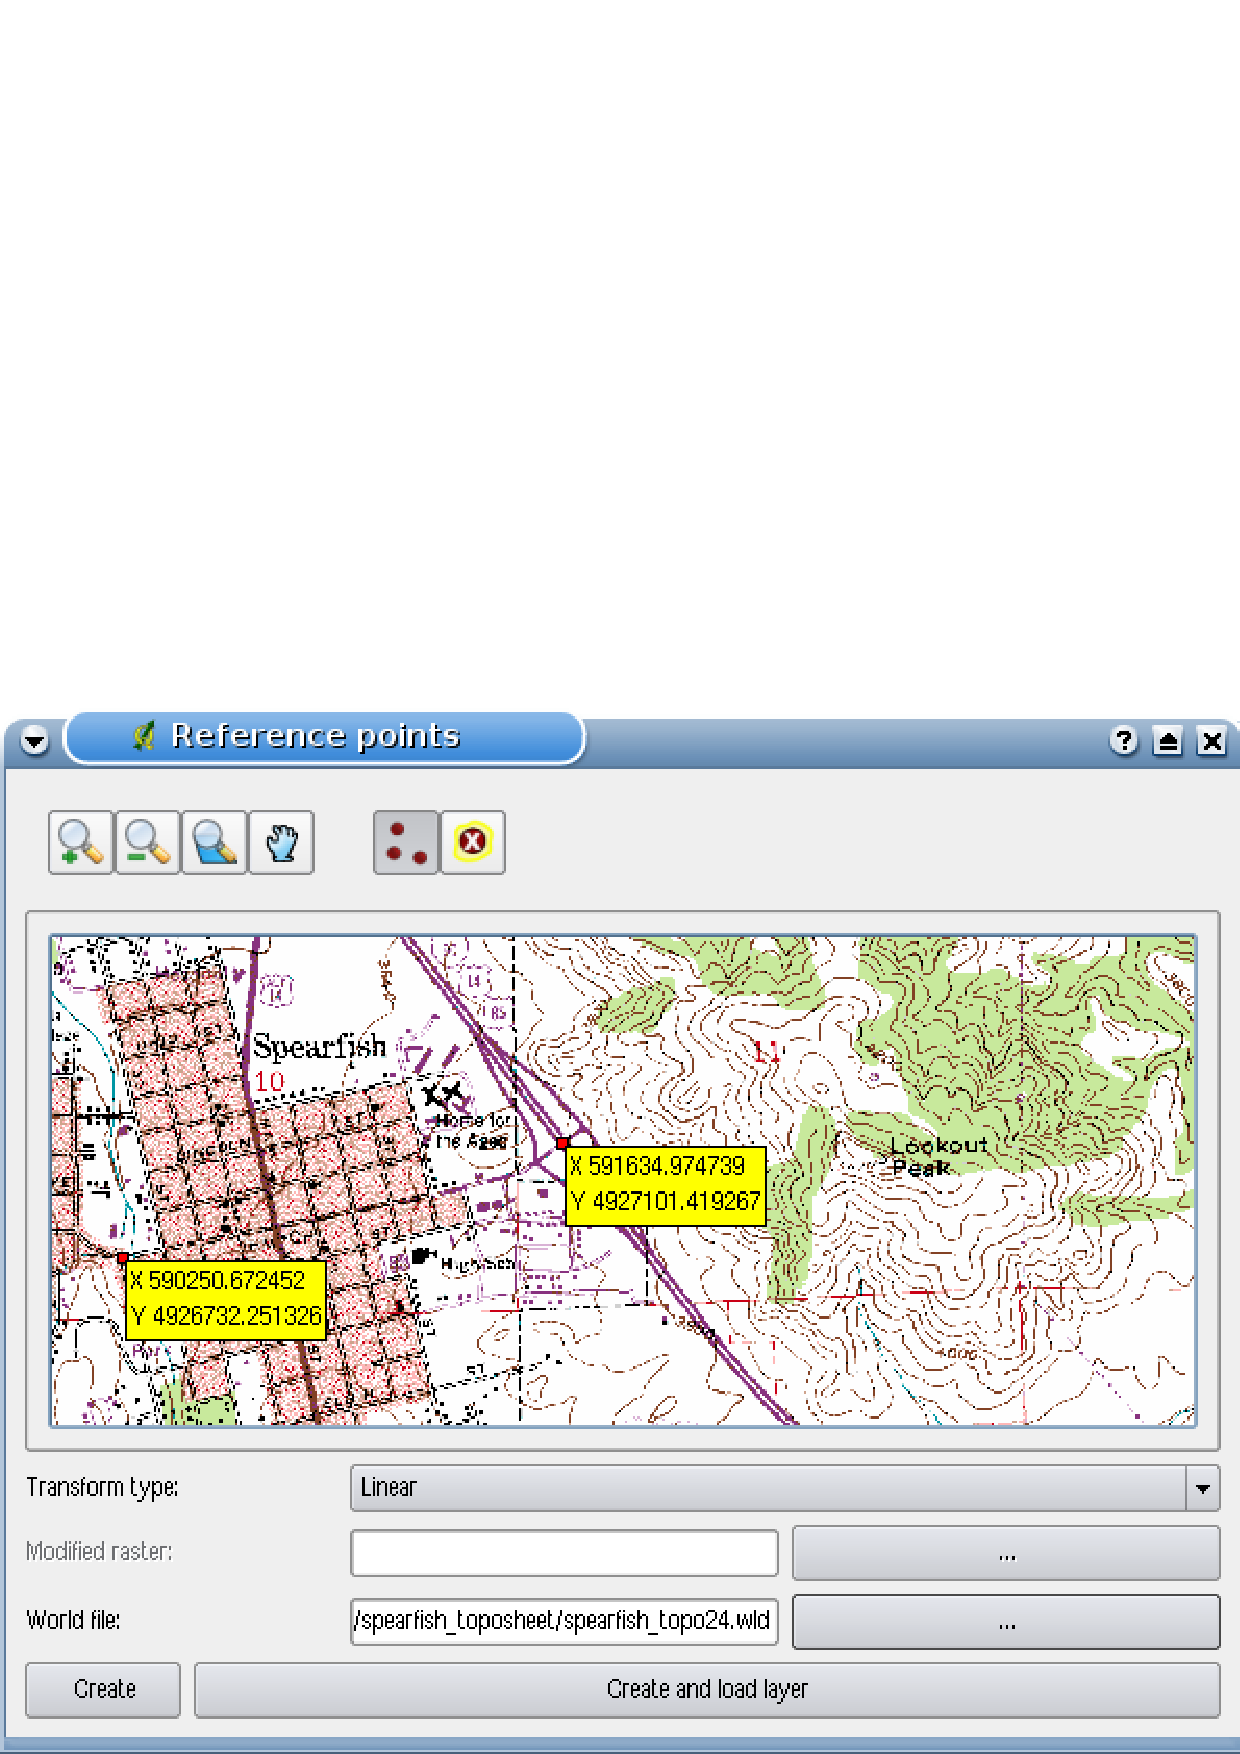
\includegraphics[clip=true,width=8cm]{choose_points}
  \caption{Coordinate di un GCP \nixcaption}\label{fig:choose_points}
\end{figure}

I punti inseriti vengono salvati in un file di testo ([filename].points), solitamente 
all'interno della cartella contenente l'immagine raster: in tal modo sarà possibile 
riaprire il plugin con gli stessi dati per aggiungere/rimuovere punti al fine di 
ottimizzare il risultato. 
Il file dei punti contiene valori nella forma: mapX, mapY, pixelX, pixelY: tali file 
possono essere gestiti con i pulsanti 
\includegraphics[width=0.7cm]{mActionFileOpen}{Carica punti GCP}
e 
\includegraphics[width=0.7cm]{mActionFileSave}{Salva punti GCP come}. 

\minisec{Impostare una trasformazione}\label{georeferencer_transformation}

Una volta aggiunti i GCP, è necessario definire le impostazioni di trasformazione del 
il processo di georeferenziazione. 

\begin{figure}[ht]
\centering
  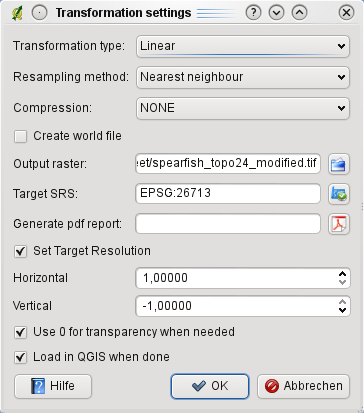
\includegraphics[clip=true,width=8cm]{transformation_settings}
  \caption{Finestra di dialogo Impostazioni di trasformazione \nixcaption}\label{fig:georef_transform}
\end{figure}

\minisec{Algoritmi di trasformazione disponibili}

Sono disponibili diversi algoritmi di trasformazione: la scelta dipende dal 
numero di GCP a disposizione, dal tipo e dalla qualità dei dati di input e 
dall'entità di distorsione geometrica che si accetta di introdurre nel 
risultato finale.

Sono disponibili i seguenti algoritmi: 

\begin{itemize}[label=--]
\item L'\textbf{Algoritmo Lineare} genera un word file, quindi non trasforma fisicamente 
il raster a differenza degli altri metodi: non è un algoritmo efficiente in caso 
di mappe provenienti da scansione di materiale cartaceo.
\item La \textbf{Trasformazione di Helmert} opera una rototraslazione.
\item Gli \textbf{Algoritmi Polinomiali} (1-3) sono molto usati: ognuno differisce in funzione 
del grado di distorsione introdotto nell'accoppiamento dei GCP. La trasformazione polinomiale 
più utilizzato è quello di secondo ordine: tiene conto della curvatura. La trasformazione 
polinomiale del primo ordine (affine) preserva la collinearità e permette la rototraslazione.
\item L'\textbf{Algoritmo Thin plate spline (TPS)} permette di introdurre deformazioni locali 
nei dati. L'algoritmo è particolarmente efficace nel caso i dati da georiferire siano di scarsa qualità.
\item La \textbf{Trasformazione Proiettiva} applica una rototraslazione delle coordinate.
\end{itemize}

\minisec{Metodo di ricampionamento}

La scelta del metodo di ricampionamento dipende dai dati in input e da alcuni requisiti utente.
Se, ad esempio, non si accettano modifiche alle statistiche dell'immagine, allora il metodo 
del vicino più prossimo sarà più adatto. Se, invece, si richiede un risultato più ``liscio'' 
(smoothed) si utilizzerà il metodo cubico.

Sono disponibili 5 diversi metodi di ricampionamento:

\begin{enumerate}
\item Vicino più prossimo
\item Lineare
\item Cubico
\item Spline cubica
\item Lanczos
\end{enumerate}

\minisec{Altre impostazioni di trasformazione}

Bisogna definire varie altre opzioni per l'output:

\begin{itemize}[label=--]
\item La casella di controllo \checkbox{Crea il file di georeferenziazione} è attiva solo
se si è scelta la trasformazione lineare, appunto quando il raster non viene fisicamente 
traformato: in tal caso, quindi, la casella Raster in output non è attiva.
\item Per tutti gli altri tipi di trasformazione bisogna definire un \textbf{Raster in output}. 
Come modalità predefinita, viene creato un nuovo file ([nomefile]\_modificato) nella 
stessa cartella del raster di partenza.
\item Bisogna, poi, scegliere il \textbf{SR} (Sistema di Riferimento) (Sezione \ref{label_projections}). 
\item Se richiesto, è possibile \textbf{generare una mappa pdf} e un \textbf{rapporto pdf}. 
Il rapporto include informazioni sui parametri della trasformazione, un'immagine dei residui, una 
lista dei GCP e degli errori RMS.
\item La casella di controllo \checkbox{Imposta risoluzione finale} permette di definire la 
risoluzione del raster di output: il valore predefinito è 1.
\item Attivando la casella di controllo \checkbox{Utilizzare 0 per la trasparenza dove necessario}, 
i pixel con valore 0 saranno trasparenti.
\item La casella di controllo \checkbox{Carica in QGIS una volta eseguito}, carica l'output nella vista 
mappa di QGIS a trasformazione terminata. 
\end{itemize}

\minisec{Proprietà del raster}

Cliccando \dialog{Proprietà del raster} nel menu \dropmenuopt{Preferenze}, si apre la finestra 
di dialogo Proprietà del layer - Raster.

\minisec{Configurare il georeferenziatore}

Cliccando \dialog{Configura il georeferenziatore} nel menu \dropmenuopt{Preferenze}, si apre 
la finestra di dialogo Configura il georeferenziatore, dove è possibile:

\begin{itemize}[label=--]
\item Definire se visualizzare coordinate e/o ID dei GCP.
\item Impostare le unità dei residui.
\item Impostare i margini per i rapporti pdf e le dimensioni per le mappe pdf.
\item Scegliere di agganciare (dock) o meno la finestra del georeferenziatore. 
\end{itemize}

\minisec{Eseguire la trasformazione}\label{georeferencer_running}

Una volta acquisiti i GCP necessari ed impostati i vari parametri della trasformazione,
cliccare su 
\includegraphics[width=0.7cm]{mActionStartGeoref}{'Inizia georeferenziazione'} 
per creare il nuovo raster georeferenziato.

